% Gallery figure source
% Summary: Four phylogenetic graph displays that should not be interpreted in the same way. A tree gives a single ancestry, an explicit phylogenetic network represents modeled reticulate ancestry, a conflict or split network displays incompatible signal, and a haplotype or median network summarizes relationships among closely related sequence types.
\documentclass[tikz,border=6pt]{standalone}
% Shared color palette
\usepackage[T1]{fontenc}
\usepackage[utf8]{inputenc}
\usepackage{lmodern}
\usepackage{microtype}
\usepackage{amsmath,amssymb,mathtools}
\usepackage{xcolor}
\usepackage{tikz}
\usetikzlibrary{arrows.meta,positioning,calc,fit,backgrounds,decorations.pathreplacing,shapes.geometric,shadows.blur}

\definecolor{mainblue}{RGB}{42,85,132}
\definecolor{deepgreen}{RGB}{30,105,70}
\definecolor{burntorange}{RGB}{190,90,25}
\definecolor{softgray}{RGB}{245,246,248}
\definecolor{darkgray}{RGB}{70,70,70}
\definecolor{violet}{RGB}{110,70,150}

\newcommand{\given}{\,|\,}
\newcommand{\Ne}{N_{e}}
\newcommand{\ARG}{\mathrm{ARG}}
\newcommand{\MRCA}{\mathrm{MRCA}}
\newcommand{\GMRCA}{\mathrm{GMRCA}}

% Shared TikZ styles
\tikzset{
  tip/.style={circle,fill=black,inner sep=1.6pt},
  nodept/.style={circle,fill=black,inner sep=1.4pt},
  sampled/.style={rectangle,fill=black,inner sep=2.2pt},
  branch/.style={line width=0.8pt},
  retic/.style={circle,draw=burntorange,fill=burntorange!25,line width=0.8pt,inner sep=2.0pt},
  event/.style={circle,draw=mainblue,fill=mainblue!15,line width=0.8pt,inner sep=1.8pt},
  arr/.style={-{Latex[length=2.0mm]},line width=0.8pt},
  faint/.style={line width=0.7pt,draw=gray!55},
  parentedge/.style={-{Latex[length=2.0mm]},line width=0.9pt,draw=burntorange},
  treeedge/.style={-{Latex[length=2.0mm]},line width=0.9pt,draw=black},
  segment/.style={line width=4pt,line cap=round},
  dashedretic/.style={-{Latex[length=2.0mm]},line width=0.9pt,draw=burntorange,dashed}
}


\begin{document}
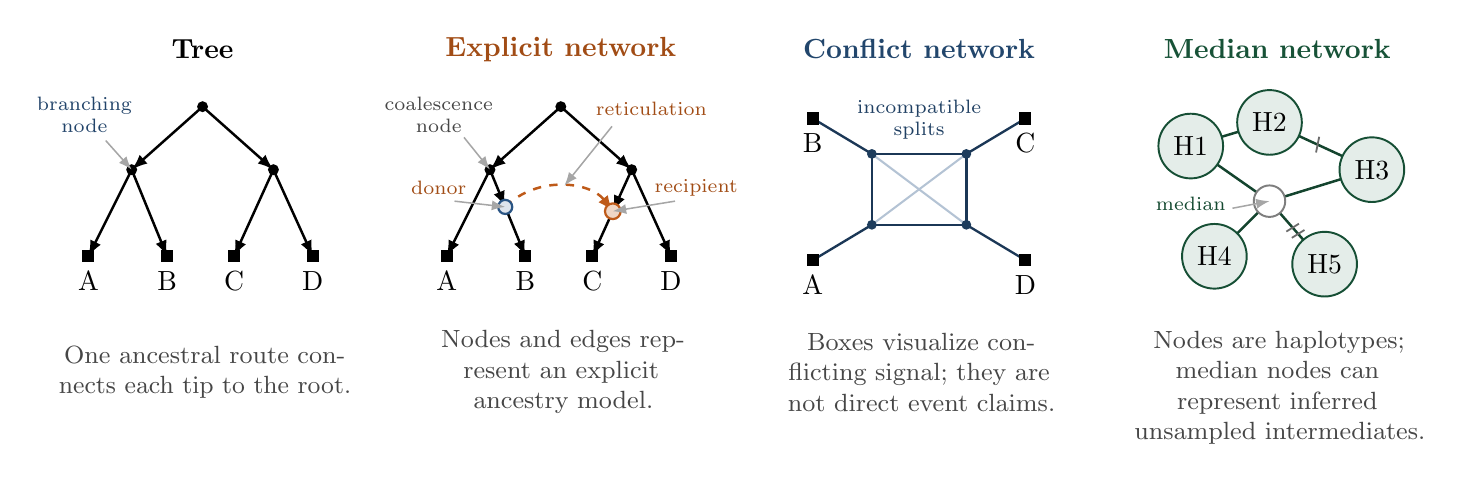
\begin{tikzpicture}[
  scale=1.0,
  paneltitle/.style={font=\bfseries},
  paneltext/.style={font=\small,align=center,text width=3.65cm,text=darkgray},
  splitline/.style={line width=.85pt,draw=mainblue!65!black},
  splitlinefaint/.style={line width=.75pt,draw=mainblue!35},
  hapedge/.style={line width=.9pt,draw=deepgreen!65!black},
  hapnode/.style={circle,draw=deepgreen!75!black,fill=deepgreen!12,line width=.7pt,minimum size=8mm},
  mediannode/.style={circle,draw=darkgray!70,fill=white,line width=.7pt,minimum size=4mm},
  smalltick/.style={line width=.65pt,draw=darkgray!80},
  callout/.style={font=\scriptsize,align=center,text=darkgray},
  callarr/.style={-{Latex[length=1.7mm]},line width=.55pt,draw=gray!70}
]

  \begin{scope}
    \node[paneltitle] at (1.65,3.38) {Tree};

    \coordinate (r)  at (1.65,2.65);
    \coordinate (n1) at (0.75,1.85);
    \coordinate (n2) at (2.55,1.85);
    \coordinate (a)  at (0.20,0.75);
    \coordinate (b)  at (1.20,0.75);
    \coordinate (c)  at (2.05,0.75);
    \coordinate (d)  at (3.05,0.75);

    \draw[treeedge] (r)--(n1);
    \draw[treeedge] (r)--(n2);
    \draw[treeedge] (n1)--(a);
    \draw[treeedge] (n1)--(b);
    \draw[treeedge] (n2)--(c);
    \draw[treeedge] (n2)--(d);

    \foreach \p in {r,n1,n2}{
      \node[nodept] at (\p) {};
    }

    \foreach \p/\lab in {a/A,b/B,c/C,d/D}{
      \node[sampled] at (\p) {};
      \node[below=2pt] at (\p) {\lab};
    }

    \node[callout,text=mainblue!80!black] at (0.15,2.55)
      {branching\\ node};
    \draw[callarr] (0.42,2.22)--(n1);

    \node[paneltext] at (1.65,-0.72)
      {One ancestral route connects each tip to the root.};
  \end{scope}

  \begin{scope}[xshift=4.55cm]
    \node[paneltitle,text=burntorange!85!black] at (1.65,3.38)
      {Explicit network};

    \coordinate (R)  at (1.65,2.65);
    \coordinate (N1) at (0.75,1.85);
    \coordinate (N2) at (2.55,1.85);
    \coordinate (A)  at (0.20,0.75);
    \coordinate (B)  at (1.20,0.75);
    \coordinate (C)  at (2.05,0.75);
    \coordinate (D)  at (3.05,0.75);

    \coordinate (donor)     at ($(N1)!0.43!(B)$);
    \coordinate (recipient) at ($(N2)!0.48!(C)$);

    \draw[treeedge] (R)--(N1);
    \draw[treeedge] (R)--(N2);
    \draw[treeedge] (N1)--(A);
    \draw[treeedge] (N1)--(donor);
    \draw[treeedge] (donor)--(B);
    \draw[treeedge] (N2)--(recipient);
    \draw[treeedge] (recipient)--(C);
    \draw[treeedge] (N2)--(D);

    \draw[dashedretic]
      (donor) .. controls (1.35,1.78) and (2.02,1.70) .. (recipient);

    \foreach \p in {R,N1,N2}{
      \node[nodept] at (\p) {};
    }

    \node[event] at (donor) {};
    \node[retic] at (recipient) {};

    \foreach \p/\lab in {A/A,B/B,C/C,D/D}{
      \node[sampled] at (\p) {};
      \node[below=2pt] at (\p) {\lab};
    }

    \node[callout,text=darkgray] at (0.10,2.55)
      {coalescence\\ node};
    \draw[callarr] (0.42,2.26)--(N1);

    \node[callout,text=burntorange!85!black] at (2.80,2.62)
      {reticulation};
    \draw[callarr] (2.30,2.40)--($(donor)!0.55!(recipient)+(0,.3)$);

    \node[callout,text=burntorange!85!black] at (0.10,1.62)
      {donor};
    \draw[callarr] (.30,1.45)--(donor);

    \node[callout,text=burntorange!85!black] at (3.37,1.62)
      {recipient};
    \draw[callarr] (3.10,1.45)--(recipient);

    \node[paneltext] at (1.65,-0.72)
      {Nodes and edges represent an explicit ancestry model.};
  \end{scope}

  \begin{scope}[xshift=9.10cm]
    \node[paneltitle,text=mainblue!82!black] at (1.65,3.38)
      {Conflict network};

    \coordinate (A) at (0.30,0.70);
    \coordinate (B) at (0.30,2.50);
    \coordinate (C) at (3.00,2.50);
    \coordinate (D) at (3.00,0.70);

    \coordinate (p1) at (1.05,2.05);
    \coordinate (p2) at (1.05,1.15);
    \coordinate (p3) at (2.25,2.05);
    \coordinate (p4) at (2.25,1.15);

    \draw[splitline] (A)--(p2);
    \draw[splitline] (B)--(p1);
    \draw[splitline] (C)--(p3);
    \draw[splitline] (D)--(p4);

    \draw[splitline] (p1)--(p3);
    \draw[splitline] (p2)--(p4);
    \draw[splitline] (p1)--(p2);
    \draw[splitline] (p3)--(p4);

    \draw[splitlinefaint] (p1)--(p4);
    \draw[splitlinefaint] (p2)--(p3);

    \foreach \p/\lab in {A/A,B/B,C/C,D/D}{
      \node[sampled] at (\p) {};
      \node[below=2pt] at (\p) {\lab};
    }

    \foreach \p in {p1,p2,p3,p4}{
      \node[circle,fill=mainblue!70!black,inner sep=1.25pt] at (\p) {};
    }

    \node[callout,text=mainblue!75!black] at (1.65,2.48)
      {incompatible\\splits};

    \node[paneltext] at (1.65,-0.72)
      {Boxes visualize conflicting signal; they are not direct event claims.};
  \end{scope}

  \begin{scope}[xshift=13.65cm]
    \node[paneltitle,text=deepgreen!78!black] at (1.65,3.38)
      {Median network};

    \coordinate (h1) at (0.55,2.15);
    \coordinate (h2) at (1.55,2.45);
    \coordinate (h3) at (2.85,1.85);
    \coordinate (h4) at (0.85,0.75);
    \coordinate (h5) at (2.25,0.65);
    \coordinate (m)  at (1.55,1.45);

    \draw[hapedge] (h1)--(h2);
    \draw[hapedge] (h2)--(h3);
    \draw[hapedge] (h1)--(m);
    \draw[hapedge] (m)--(h3);
    \draw[hapedge] (m)--(h4);
    \draw[hapedge] (m)--(h5);

    \draw[smalltick] ($(h2)!0.47!(h3)+(0.02,0.10)$)--($(h2)!0.47!(h3)+(-0.02,-0.10)$);
    \draw[smalltick] ($(m)!0.42!(h5)+(0.08,0.05)$)--($(m)!0.42!(h5)+(-0.08,-0.05)$);
    \draw[smalltick] ($(m)!0.52!(h5)+(0.08,0.05)$)--($(m)!0.52!(h5)+(-0.08,-0.05)$);

    \node[hapnode,minimum size=6mm] at (h1) {H1};
    \node[hapnode,minimum size=3.5mm] at (h2) {H2};
    \node[hapnode,minimum size=5mm] at (h3) {H3};
    \node[hapnode,minimum size=5mm] at (h4) {H4};
    \node[hapnode,minimum size=4mm] at (h5) {H5};
    \node[mediannode] at (m) {};

    \node[callout,text=deepgreen!70!black] at (0.55,1.42)
      {median};
    \draw[callarr] (1.08,1.36)--(m);

    \node[paneltext] at (1.65,-0.92)
      {Nodes are haplotypes; median nodes can represent inferred unsampled intermediates.};
  \end{scope}
\end{tikzpicture}
\end{document}
